\documentclass[10pt]{article}
\usepackage{mathtools}
\usepackage{amssymb}
\usepackage{amsthm}
\usepackage{hyperref}
\usepackage{graphicx}


\title{Particle Filter (assignment 1)}
\author{Yi Tian Xu\\260520039}


\begin{document}
\maketitle

\section{Initialization}
At the beginning, I create $n=400$ particles. Each particles is assigned with a random $x$ and $y$ coordinate according to the uniform distribution, and a random angle $\theta$ according to the Gaussian distribution. The weight for each particle is initialized with the inverse of the total number of particles. This can ensure that the initial hypothesis of the robot's position is not biased by regions that have more particles or by particles that have more weights. 

\section{Motion Model}
Each time when the robot makes a move, each particle $p$ is replaced by a new particle $p'$ sampled from $p(s'|u_{t-1}, s)$ where $s' = (x', y', \theta')$ is the new position of the particle, $u_{t-1}$ is the action taken at time $t-1$ and $s = (x, y, \theta)$ is the previous position of the particle. I assumed that this distribution is Gaussian with mean and standard deviation as follows:
\begin{align*}
	&\mu = s + \delta \\ 
	&\sigma = (0.1, 0.1, 0.1)
\end{align*}
where $\delta$ represent the values from the odometer after taking action $u_{t-1}$. I also assume that $X$, $Y$, $\Theta$ are independent random variables distributed normally. 

The weight of the new particle is the same as the old one. 

\subsection{Design Decisions}
In a previous design, the standard deviation was chosen to match the \texttt{odom\_error} in \texttt{lab.world} file. However, after doing some tests and observed the , it seems that arbitrary choices for the standard deviation that are consistent with the odometer's measurements are good enough to simulate the noise. 

\section{Sensor Model}
The weight of particles is updated based on the data that the robot receives with its laser sensor. To do so, a simulation of the received data is done for each particle, and the ``distance" between each simulated data point with the true data point is used to calculate the new weight. 

Since the object \texttt{sensor\_msgs/LaserScan} in ROS has the data array sorted by the angle of the laser scan, I calculate the new belief as follows. Given a simulated sequence of ranges $R^{(p)}_n = (r^{(p)}_1, r^{(p)}_2, \dots, r^{(p)}_n)$ at the position of some particle $p$, and the true sequence $R_n = (r_1, r_2, \dots, r_n)$,
\begin{displaymath}
	p(z|s) = p(S_n|p) = \alpha\sum_{i=1}^n \exp\left(-\frac{\left(r^{(p)}_i - r_i\right)^2}{l^2}\right)
\end{displaymath}
where $l$ is a constant, and $\alpha$ is the normalization factor. Now, the new weight of particle $p$ is  
\begin{displaymath}
	w' = p(z|s)w
\end{displaymath}
where $w$ is the old weight. 

\subsection{Design Decisions}
For time efficiency, I tried to compare the minimum and maximum ranges between the simulated and true data before deciding to compare all the ranges. I proposed that if this comparison shows that there is a significant difference, i.e.: if the difference between minimum or maximum ranges is above a certain threshold, then I set the new weight to zero. However, the choice of the threshold was unclear. Moreover, in some circumstances, this heuristic wipes out many particles that are near the true position and allocates many new particles at some other places that happens to have similar minimum and maximum ranges but with different order. So I removed this heuristic. 

Another issue that I encountered was underflow when preforming 
$[p(z|s)/\alpha]w$. Since I can only normalize at the end in my implementation, I decided to use $(1-w)^{-1}$ instead of $w$, and adjust the normalizing factor accordingly.

\section{Resampling}
To avoid degeneracy, I take away particles with low weight and  add new particles near particles that are heavier. The resampling algorithm that I used was found in the paper by Arulampalam et al. in 2002 \cite[p. 180]{paper}. In this algorithm, we first check if the effective sample size, $N_{eff}$, is smaller than some $N_T$. This indicate whether there's severe degeneracy. If there is, we then we estimate the cumulative distribution function (CDF) of the weights using the weights themselves as probabilities, which can be easily done since the weights were normalized in the sensor model. 

Defining a quantile $q_{\nu_i}$ to be the section in the CDF such that $p(W > w) < \nu_i$ for some weight $w$. The algorithm chooses $n$ new particles such that each there is at most $i$ particles with weight in quantile $q_{\nu_i}$, $\nu_i\in \{u +n^{-1}*(i-1)\}$, where $u$ is drawn from uniform distribution on the interval $[0, n^{-1}]$.

\subsection{Design Decisions}
The algorithm assign each of the new particles with the same position than the first particle whose weight is above the smallest quantile that the new particle corresponds to. I thought that, in the case there is a lot of degeneracy, it may happen that some particle is so heavy that it is the only closest representative above some consecutive quantiles. So I used Gaussian distribution centered at the old particle's position to add more dispersion.
 
\section{Estimate Update}
As the density of the particles now describes the significance of the region where they are allocated to, I defined the new estimate to be the sample mean.
\begin{displaymath}
	\bar{s} = \frac{1}{n}\sum_{p} s^{(p)}
\end{displaymath}
Since I assumed that $X$, $Y$, $\Theta$ are independent, the covariance matrix is a diagonal matrix. I used the sample variance to estimate it. 

\subsection{Design Decisions}
As $n$ is large, the sample variance becomes
\begin{displaymath}
	\hat{\sigma}_s = \frac{1}{n-1}\sum_{p}(s^{(p)}-\bar{s})^2 \approx \frac{1}{n}\sum_{p}(s^{(p)}-\bar{s})^2
\end{displaymath}
So to simplify the computation, I used the formula on the right hand side to approximate the estimate. 

Furthermore, since $\bar{s}$ must be known before computing the variance, I used the previous estimate to avoid making another loop in the program. 

\section{Performance}
My implementation is able to estimate the robot's location with a high standard deviation within a reasonable time. Occasionally the estimated position matches closely to the robot's true location and orientation. 

When particles converges to a region on the map, they may disperse again when the robot quickly moves to another location. 

\begin{figure}[ht!]
\centering
\advance\leftskip-3cm
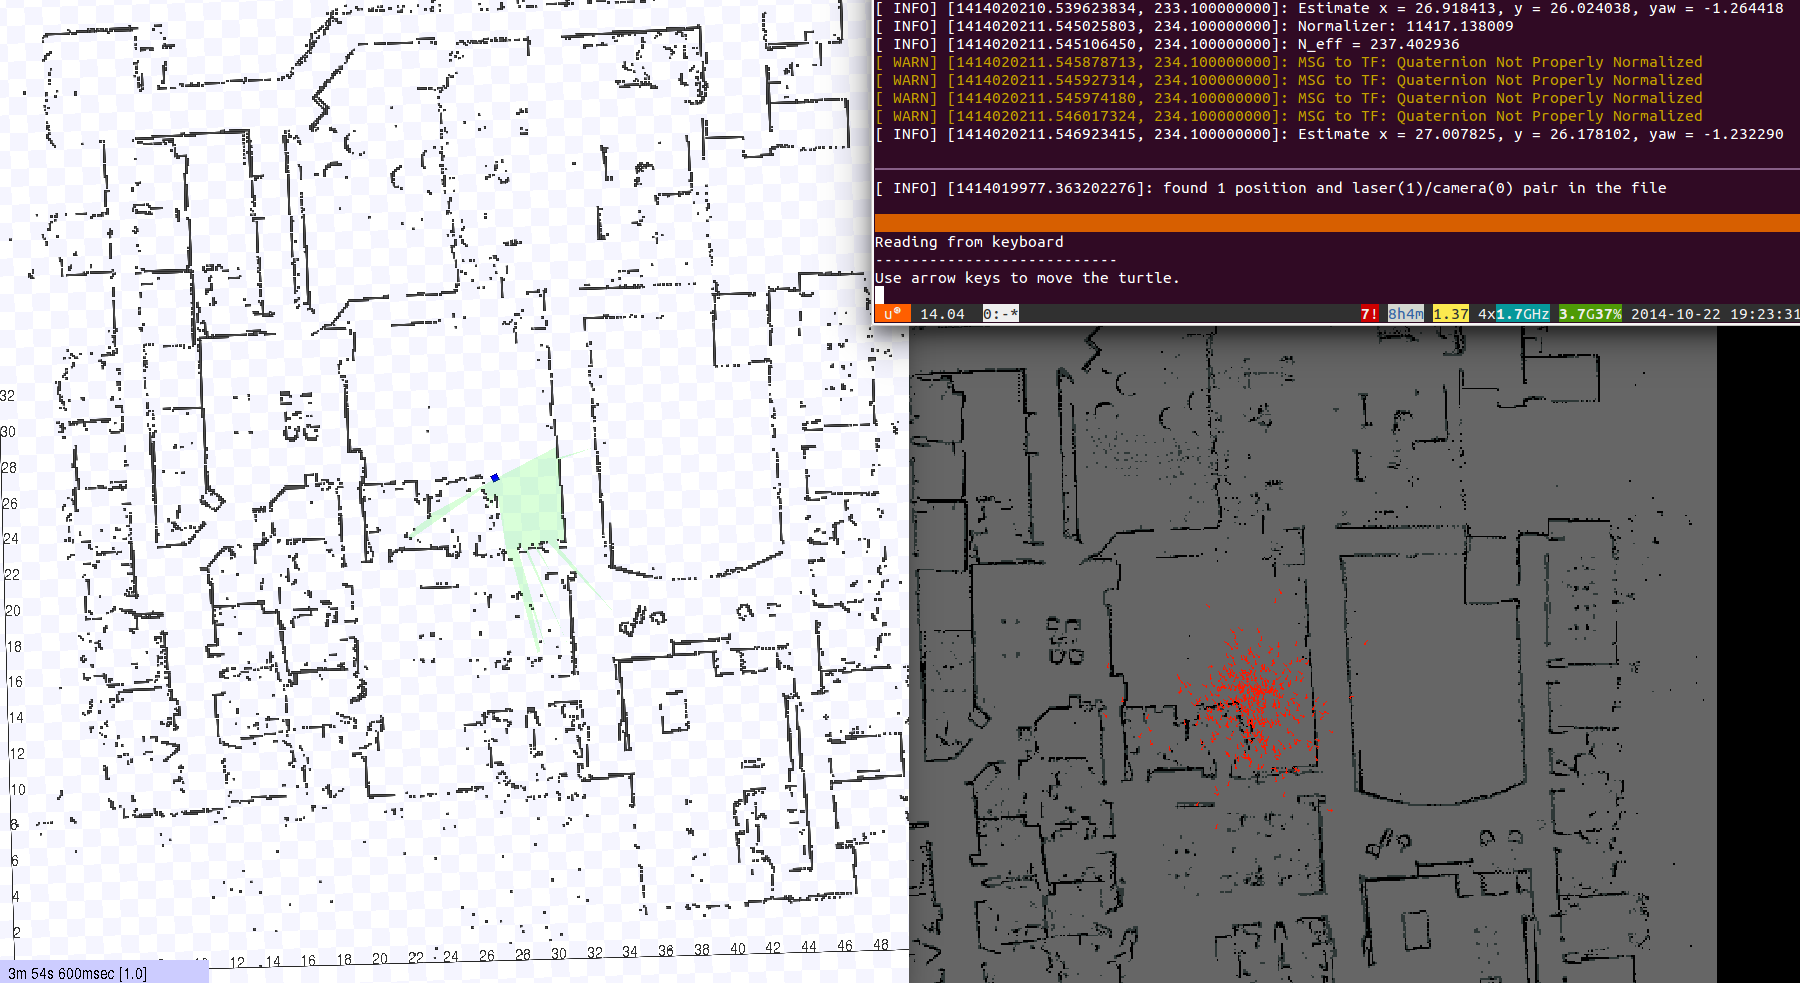
\includegraphics[width=180mm]{pic.png}
\caption{The particles converging at $s \approx (27,26,-1.23)$.}
\label{figCir1}
\end{figure}

\section{Improvements}
Often, the particles may converge to a region on the map that is not the true location of the robot. This happens when there are many locations scattered on the maps that look similar for the robot, resulting local maxima in the space of distribution functions of the particles. To jump out of those local maxima, we can consider adding random restart algorithm. 

Aside from adding more features, the choice for the number of particles ($n$), the odometer's standard deviation ($\sigma$), the threshold for the effective sample size ($N_T$) and the constant in the sensor model ($l$) can be further explored and optimized to improve the performance of this algorithm. 


\begin{thebibliography}{9}

\bibitem{paper}
  M. Sanjeev Arulampalam, Simon Maskell, Neil Gordon, and Tim Clapp
  \emph{A Tutorial on Particle Filters for Online
Nonlinear/Non-Gaussian Bayesian Tracking}.
  IEEE Transactions on Signal Processing, vol. 50, no. 2, 
  February 2002. $<$\url{http://www.cse.psu.edu/~rcollins/CSE598G/papers/ParticleFilterTutorial.pdf}$>$
\end{thebibliography}
\end{document}
